\documentclass[submit]{harvardml}

\course{CS181-S20}
\assignment{Assignment \#4}
\duedate{11:59pm March 27, 2020} 

\usepackage[OT1]{fontenc}
\usepackage[colorlinks,citecolor=blue,urlcolor=blue]{hyperref}
\usepackage[pdftex]{graphicx}
\usepackage{graphicx}
\usepackage{caption}
\usepackage{fullpage}
\usepackage{soul}
\usepackage{amsmath}
\usepackage{amssymb}
\usepackage{color}
\usepackage{todonotes}
\usepackage{listings}
\usepackage{common}

\usepackage[mmddyyyy,hhmmss]{datetime}

\definecolor{verbgray}{gray}{0.9}

\lstnewenvironment{csv}{
  \lstset{backgroundcolor=\color{verbgray},
  frame=single,
  framerule=0pt,
  basicstyle=\ttfamily,
  columns=fullflexible}}{}
 
\begin{document}

\begin{center}
{\Large Homework 4: SVM, Clustering, and Ethics}\\
\end{center}

\subsection*{Introduction}

This homework assignment will have you work with SVMs, 
clustering, and engage with the ethics lecture.  

Please submit the \textbf{writeup PDF to the Gradescope assignment `HW4'}. Remember to assign pages for each question.

Please submit your \textbf{\LaTeX\ file and code files to the Gradescope assignment `HW4 - Supplemental'}. 

You can use a \textbf{maximum of 2 late days} on this assignment.  Late days will be counted based on the latest of your submissions. 

\newpage

%%%%%%%%%%%%%%%%%%%%%%%%%%%%%%%%%%%%%%%%%%%%%
% Problem 1
%%%%%%%%%%%%%%%%%%%%%%%%%%%%%%%%%%%%%%%%%%%%%
\begin{problem}[Fitting an SVM by hand, 10pts]

  For this problem you will solve an SVM by hand, relying on principled rules and SVM properties. 
  For making plots, however, you are allowed to use a computer or other graphical tools.

Consider a dataset with the following 7 data points each with $x \in \reals$ and $y \in \{ -1, +1 \}$ : \[\{(x_i, y_i)\}_{i = 1}^7 =\{(-3 , +1) , (-2 , +1 ) , (-1,  -1 ), (0, +1), ( 1 , -1 ), ( 2 , +1 ) , (3 , +1 )\}\] Consider
mapping these points to $2$ dimensions using the feature vector $\bphi(x) =  (x, -\frac{8}{3}x^2 + \frac{2}{3}x^4 )$. The hard margin classifier training problem is:
%
\begin{align*}
  &\min_{\mathbf{w}, w_0} \|\mathbf{w}\|_2^2 \label{eq:dcp} \\
  \quad \text{s.t.} \quad & y_i(\mathbf{w}^\top \bphi(x_i) + w_0) \geq 1,~\forall i \in \{1,\ldots, n\}\notag
\end{align*}

Make sure to follow the logical structure of
the questions below when composing your answers, and to justify each step.

\begin{enumerate}
\item Plot the transformed training data in $\reals^2$ and draw the optimal decision boundary
of the max margin classifier. You can determine this by inspection (i.e. by hand, without actually doing any calculations).

\item  What is the value of the margin achieved by the optimal
decision boundary found in Part 1? 

\item Identify a unit vector that is orthogonal to the decision boundary.

\item Considering the discriminant $h(\bphi(x);\boldw,w_0)=\boldw^\top\bphi(x) +w_0$, 
give an expression for {\em all possible} $(\boldw,w_0)$ that define
the decision boundary. Justify your answer.

  \item Consider now the training problem for this dataset. Using your answers so far,
    what particular solution to $\boldw$ will be optimal for the
    optimization problem?

  \item What is the corresponding optimal value of $w_0$ for the $\boldw$ found in Part 5 (use your result from Part 4 as guidance)? Substitute in these optimal values and write out the discriminant function
    $h(\bphi(x);\boldw,w_0)$ in terms of the variable $x$ .


\item What are the support vectors of the classifier?  Confirm that
  the solution in Part 6 makes the constraints above binding for these
  support vectors.

\end{enumerate}

\end{problem}

\subsection*{Solution}
\begin{enumerate}
    \item 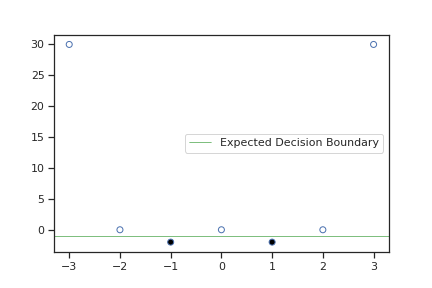
\includegraphics{cs181-s20-homeworks/hw4/ExpectedBoundary.png}
    \item The margin is 1
    \item A unit vector that is orthogonal to the decision boundary is 
        \begin{bmatrix}
           0 \\
           1 \\
         \end{bmatrix}.
    \item To solve for $w_0$ we could set the discriminant function to 0 and input the unit vector we found in question 3. Alternatively, any unit vector orthogonal to the decision boundary is a valid value for $\boldw$.\\

    Given this truth for $\boldw$, let $\boldw = \begin{bmatrix}
           0 \\
           \alpha \\
         \end{bmatrix}$ where $\alpha \in \reals$. We can plug this value of $\boldw$ into the discriminant function to find that:  
        \begin{equation}
                \begin{split}
                    h(\bphi(x);\boldw, w_0) &= \boldw^T \begin{bmatrix} 
                    0 \\
                    -1 \\
                    \end{bmatrix} + w_0 = 0\\
                    &= \begin{bmatrix} 
                    0 &
                    \alpha \\
                    \end{bmatrix}
                     \begin{bmatrix} 
                    0 \\
                    -1 \\
                    \end{bmatrix} + w_0 = 0 \\
                    w_0 &= \alpha
                \end{split}
            \end{equation} \\
         
         Further, we know that we can multiple both parameters by any constant and it's still a solution because scaling doesn't affect the relative distance from the decision boundary.
         \\
\item 
    For $\bphi(x_i)$ we can use any given value of $x$ that is close to the decision boundary, so I will use \begin{bmatrix}
    0 \\
    0\\
    \end{bmatrix}. From the previous question we know that $w_0 = \alpha$ and $\boldw = \begin{bmatrix}
    0\\
    \alpha \\
    \end{bmatrix}$. Using this we can use the hard margin classifier training problem to solve for $\boldw^*$:
        \begin{align*}
          &\min_{\mathbf{w}, w_0} \|\mathbf{w}\|_2^2 \label{eq:dcp} \\
          \quad \text{s.t.} \quad &
          y_i(\mathbf{w}^\top \bphi(x_i) + w_0) \geq 1,~\forall i \in \{1,\ldots, n\}\notag \\
            \quad & y_i(\begin{bmatrix}
            0 & \alpha \\
            \end{bmatrix} \begin{bmatrix}
            0 \\
            0\\
            \end{bmatrix} + \alpha) \geq 1
            \label{eq:dcp} \\
            \quad &
            y_i(0+\alpha) \geq 1
        \end{align*}

    The $\alpha$ that minimizes this function is 1. So, $\boldw^* =    \begin{bmatrix}
           0 \\
           1 \\
         \end{bmatrix}$ \\
\item 
    Given the answers from the previous problems, the $\alpha$ that minimizes this problem is 1. \\
    Therefore, $w_0^* = 1$
\item
    The support vectors of the classifier are all of the values of $\bphi(x)$ that are closest to the classification boundary. In this case this would be \begin{bmatrix}
    -2 & -1 & 0 & 1 & 2 \\
    0 & -2 & 0 & -2 & 0 \\
    \end{bmatrix}. When plugged into the above expression, all of these vectors satisfy the constraint.
    
\end{enumerate}
% \newpage

%%%%%%%%%%%%%%%%%%%%%%%%%%%%%%%%%%%%%%%%%%%%%
% Problem 2
%%%%%%%%%%%%%%%%%%%%%%%%%%%%%%%%%%%%%%%%%%%%%

\begin{problem}[K-Means and HAC, 20pts]


For this problem you will implement K-Means clustering and HAC from
scratch. Using \texttt{numpy} is fine, but don't use a third-party
machine learning implementation like \texttt{scikit-learn}. You will
then apply this approach to the clustering of image data.

We've provided you with a subset of the MNIST dataset, a collection of
handwritten digits used as a benchmark for image recognition (you can
learn more about the data set at
\url{http://yann.lecun.com/exdb/mnist/}). The MNIST task is widely
used in supervised learning, and modern algorithms do very well.

Here you will apply unsupervised learning to MNIST. You have been given
representations of MNIST images, each of which is a $784\times1$
greyscale handwritten digit from 0-9. Your job is to implement K-means
clustering and HAC on MNIST, and to test whether these relatively
simple algorithms can cluster similar-looking images together.

The code given in \texttt{T4\_P2.py} loads the images into your environment into two arrays -- \texttt{large\_dataset} is a 5000x784 array that should be used for K-means, while \texttt{small\_dataset} is a 300x784 array that will be used for HAC clustering. In your code, you should use the $\ell_2$ norm (i.e. Euclidean distance) as your distance metric.

\textbf{Important:} Remember to include all of your plots in your PDF submission!

\begin{enumerate}

\item Starting at a random initialization and $K = 10$, plot
  the K-means objective function (the residual sum of squares) as a function of iterations and verify
  that it never increases.

\item Run the K-means algorithm for 5 different restarts for different
  values of $K$, setting $K = 5, 10, 20$. Plot the final K-means objective value as a function
  of $K$ with error bars over the $5$ random restarts. To clarify, your
  x-axis will be $K$, your y-axis will be the average objective function value
  after your algorithm converges, and each data point will have an
  error bar -- to calculate these error bars you must run your K-means
  algorithm $5$ times for each $K$ (giving you multiple final objective values
  for each $K$) then use these values to calculate a standard deviation for
  each $K$ before plotting error bars around each data point. How
  does the final value of the objective function and the standard deviation of the final
  value of the objective function change with $K$? (Note: Our code takes ~10 minutes to run for this Part)
  
\item For $K=10$ and for 5 random restarts, show the mean
  image (aka the centroid) for each cluster.
  To render an image, use the pyplot
  \texttt{imshow} function. There should be 50 total images. Include all of these images
  as part of a single plot (e.g. don't have 50 pages in your write-up with a
  separate image on each page).

\item Repeat Part 3, but first standardize the data. That is, center
  the data before running K-means on it, such that each pixel has mean 0 and variance 1 (except
  for any pixels that have zero variance, for these you can simply
  divide by 1). For $K=10$ and 5 random restarts, show the mean image
  (aka the centroid) for each cluster. There should be 50 total
  images. Again, include all of these images as part of a single plot.
  Compare these images to those from Part 3.

\item Implement HAC for min, max, and centroid-based linkages. Fit these models to the \texttt{small\_dataset} images. 
  For each of these 3 linkage criteria, find the mean image for each cluster when using $10$ clusters, and display these images on a plot. There should be 30 total images.
  How do these mean images compare to those found with K-means? \textbf{Important Note:} For this part only, you may use the \texttt{scipy} package's \texttt{cdist} function to calculate the Euclidean distances between every pair of points in two arrays. DO NOT use \texttt{scipy} for anything else. 

\item For each of the 3 HAC linkages (max/min/centroid), make a plot of
  ``Distance between most recently merged clusters" (y-axis) v. ``Total number of merges completed" (x-axis).
  Does this plot suggest that there are any  natural cut points? 

\item Re-fit a K-means with $K = 10$ model and HAC min/max/centroid models using $10$ clusters on the \texttt{small\_dataset} images. Use the \texttt{seaborn} module's \texttt{heatmap} function to plot a confusion matrix of clusters v. actual digits, i.e. the cell at the $i$th row, $j$th column of your confusion matrix should be the number of times that an image with the true label of $j$ appears in cluster $i$. How well do the different approaches match the digits? Is this matching a reasonable evaluation metric for the clustering?  Explain why or why not.  
  
\end{enumerate}

\end{problem}

\subsection*{Solution}
\begin{enumerate}
    \item 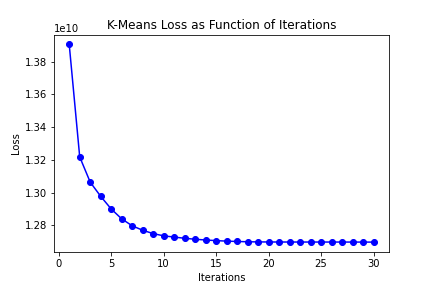
\includegraphics[scale=1]{cs181-s20-homeworks/hw4/LossIters.png}\\
    \item 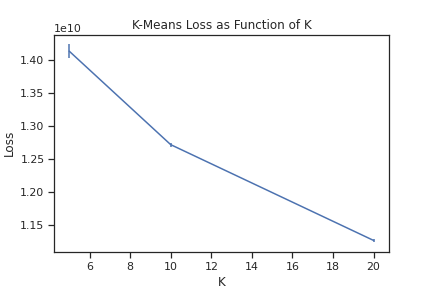
\includegraphics[scale=1]{cs181-s20-homeworks/hw4/LossKRestarts (1).png}\\
    As K increases, the loss decreases and the error bars shrink as well. This makes sense because as the number of clusters increases, the number of points in them decreases and eventually each cluster will contain one point, which would result in zero loss.
    \item 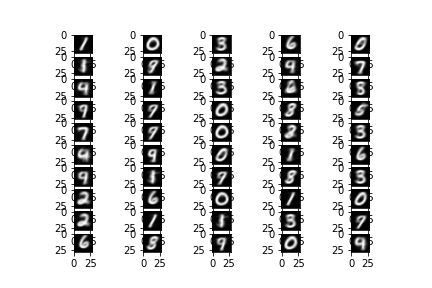
\includegraphics[scale=.9]{cs181-s20-homeworks/hw4/means .png}\\
    \item 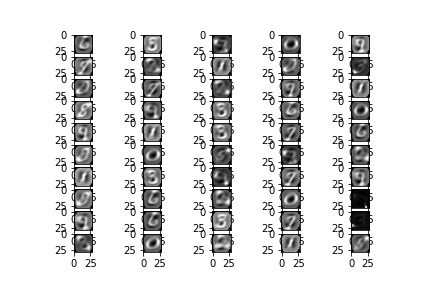
\includegraphics[scale=.9]{cs181-s20-homeworks/hw4/standardized_means2 (1).png} \\
    The standardized data does cluster as well as the non-standardized data. This is because when you standardize the data, you increase the "importance" of all the features so that they weigh similarly on the clustering decision. However, in a data set like this where many of the features are not important (i.e. mostly black space in the images that gives us little information), this reduces the precision of the mean image. Instead of having crisp boundaries between black backgrounds and white boundaries, we now have much more gray space, which renders the mean image blurry.\\
    \item
    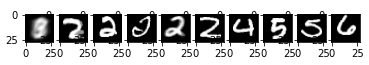
\includegraphics[scale=.7]{cs181-s20-homeworks/hw4/HAC_Minimum.png}\\
    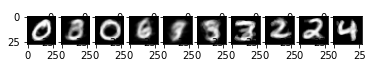
\includegraphics[scale=.7]{cs181-s20-homeworks/hw4/HAC_Maximum.png} \\
    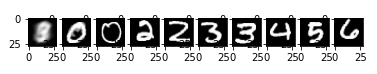
\includegraphics[scale=.7]{cs181-s20-homeworks/hw4/HAC_Centroid.png} \\
    These mean images are less interpretable, meaning they do not clearly match with digits they are supposed to represent. There are also fewer variations between digits, meaning not every digit 0-9 has a clear cluster and some digits are represented across multiple clusters. As such, we can see that HAC does a poor job of clustering compared to the K-means algorithm.
    \item 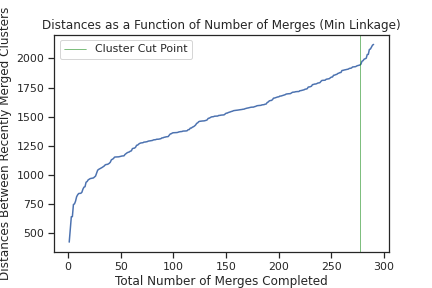
\includegraphics[scale=.6]{cs181-s20-homeworks/hw4/MergeCountsMin (3).png}\\
    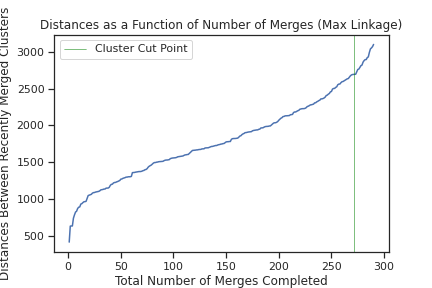
\includegraphics[scale=.6]{cs181-s20-homeworks/hw4/MergeCountsMax (1).png}\\
    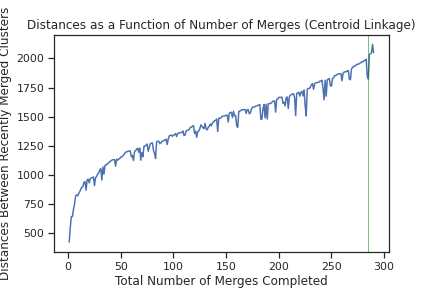
\includegraphics[scale=.6]{cs181-s20-homeworks/hw4/MergeCountsCent (1).png}\\
    As portrayed in these graphs, it appears that the natural cut point for each model is between 270-285 merges; however, this is hard to determine because there are no drastic increases in any of the plots. The most drastic increase is in the Min Linkage plot (at around 280 merges). When inspected further, I found that the first cluster in this model has 285 points which is reflected by this natural cut point in the graph. 
    \item 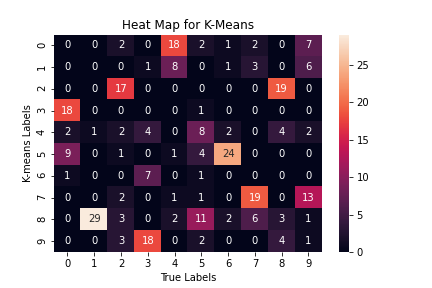
\includegraphics[scale=.6]{cs181-s20-homeworks/hw4/Kmeans_Confusion.png}\\
    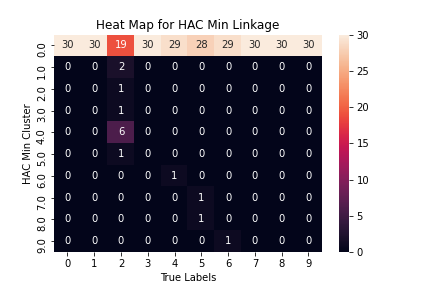
\includegraphics[scale=.6]{cs181-s20-homeworks/hw4/HAC_Min_Confusion.png}\\
    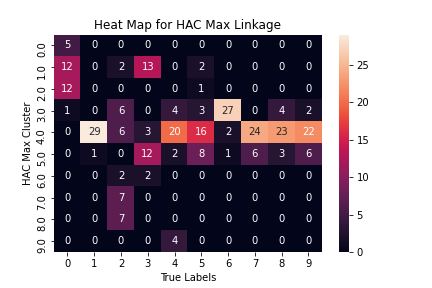
\includegraphics[scale=.6]{cs181-s20-homeworks/hw4/HAC_Max_Confusion.png}\\
    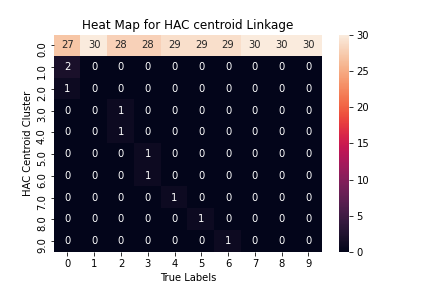
\includegraphics[scale=.6]{cs181-s20-homeworks/hw4/HAC_Centroid_Confusion.png}\\
    At a high level, k-means is a top down algorithm, where HAC is bottom up algorithm. We know there are 10 clear classes (digits 0-9), so it makes more sense to use a top down paradigm (K-Means) because it more closely corresponds to how the data were generated. This is reflected in the confusion maps quite clearly. For example, in the HAC min linkage and centroid linkage confusion matrices, we see that all of the digits were classified in the first cluster, meaning the model did not accurately identify and cluster any of the digits. The HAC max linkage confusion matrix shows that several digits were consistently classified among several clusters, which is slightly better; however, cluster 4 had the majority of points and 6 different digits were included at high rates in that particular cluster. The K-means confusion matrix shows that most digits had a clear cluster in which they dominated, and that those clusters were distinct from other clusters. Exceptions to this trend include clusters 1 (which struggled to distinguish 4's from 9's), 7 (which struggled to distinguish 7's and 9's), and 8 (which struggled to distinguish 1's from 5's). Given these findings, and the fact that they seem to match with what we can observe in the mean image plots, I would say that matching is a useful metric for success.\\
\end{enumerate}

\newpage
%%%%%%%%%%%%%%%%%%%%%%%%%%%%%%%%%%%%%%%%%%%%%
% Problem 3
%%%%%%%%%%%%%%%%%%%%%%%%%%%%%%%%%%%%%%%%%%%%%
\begin{problem}[Ethics Assignment, 15pts]
Imagine that you are a product manager in a technology company and the board of directors requests a detailed report of the potential social impact of the product you're building. You are currently working on an algorithm designed to allocate economic resources for various health providers. You are instructed to address various kinds of possible impacts, giving special attention to the algorithm’s potential to wrongfully discriminate against vulnerable populations. 

Having followed the coding process closely, you can confidently assume that there is no discriminatory intent animating the design.  In fact, the product’s design is based on the notion that resources should be distributed to health centers in a manner that is proportional to the needs of the populations they attend to. However, you worry that there may still be wrongful discrimination due to disparate negative impact on members of low-income populations, migrants, and racial minorities. 

What further questions must you address in order to confidently determine whether the algorithm wrongfully discriminates against members of these groups? Write two questions and, for each, write a short paragraph explaining how addressing this question can help you assess the algorithm’s potential for wrongful discrimination.


We expect clear, concise, and thoughtful engagement with this question, which includes providing your reasoning for your answers.  In your response, depth is more important than breadth. We do \emph{not} expect you to do any outside research, though we encourage you to connect to lecture materials where relevant.

\end{problem}

\subsection*{Solution}
\\
The first question to address would be: What is the ground truth we are measuring against and what sorts of biases exist in the model's training data? \\

Even if no statistical bias is found in the algorithm's outputs and therefore there is no disparate treatment, the system may still perpetuate unfairness if there are distortions or biases in the data used for modeling (i.e., disparate impact). One example of what this might look like is that health care providers that predominantly service low-income, migrant, communities of color, or other protected categories of users have historically been underfunded relative to their peers in more affluent or white communities, and therefore the model assumes that this is a feature that should be used to make future predictions. Without an evaluation and explicit acknowledgement of this fact, our algorithm may be unwittingly perpetuating these historical biases. \\

The second question to address would be: How robust is the algorithm to outside attacks? In other words, is it possible for some health providers to game the algorithm? \\

Because financial resources are scarce in nature, we can assume that a nontrivial number of bad actors will work in unethical ways to game our system to their advantage. Because of this, we should pressure test our program to see if there exist any ways for better resourced providers–or more sophisticated agents–to influence the outcomes by inputting embellished or falsified data. This is likely to disproportionately impact under resourced providers who disproportionately serve marginalized communities because they likely have fewer resources to deconstruct the nature of the algorithm and exploit it to their advantage. 

\newpage
%%%%%%%%%%%%%%%%%%%%%%%%%%%%%%%%%%%%%%%%%%%%%
% Name and Calibration
%%%%%%%%%%%%%%%%%%%%%%%%%%%%%%%%%%%%%%%%%%%%%
\subsection*{Name}

\subsection*{Collaborators and Resources}
Whom did you work with, and did you use any resources beyond cs181-textbook and your notes?\\

Ife, John Tucker, Luis V., Michele Wang, Cindy, 
Guillermo, Edward, Office Hours.

\subsection*{Calibration}
Approximately how long did this homework take you to complete (in hours)? \\

~15

\end{document}
